\renewcommand{\thechapter}{\Roman{chapter}}
\chapter{Methodology}
\renewcommand{\thechapter}{\arabic{chapter}}
\label{ch3:Methodology}
\thispagestyle{empty}

In this chapter, the study discusses the systematic approach employed in the development of of the proposed system. As depicted in Figure \ref{ch3:fig:system_development_process}, each phases is essential in shaping the overall system functionality. This chapter explains the approach taken, giving an overview of the techniques, methods, and resources applied at every development step.

\begin{figure}[H]
	\centering
	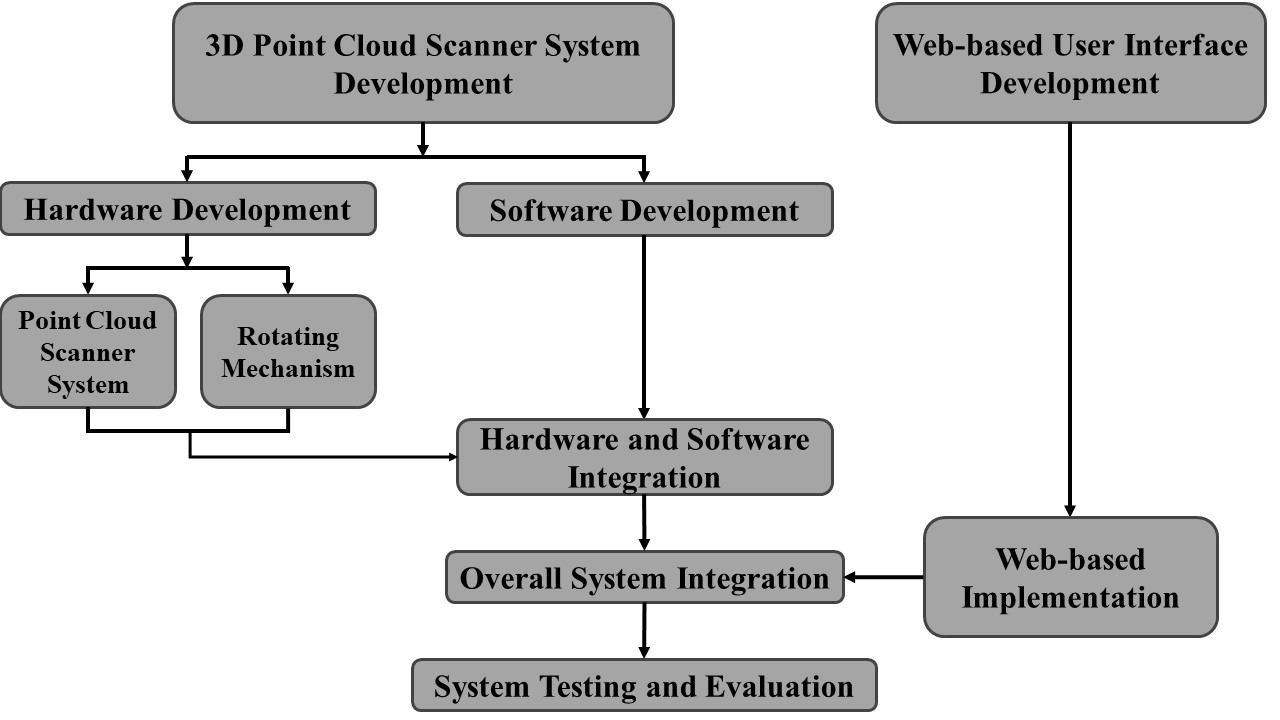
\includegraphics[width=1\textwidth]{Figures/system_development_process}
	\caption{System Development Process}
	\label{ch3:fig:system_development_process}
\end{figure}

\section{System Requirements Analysis}
\label{ch3:sec:system_requirements_analysis}

The development process of the study encompasses hardware, software, and web-based application design, followed by system integration and testing. As depicted in Figure \ref{ch3:fig:overall_system_setup_development} which is the proposed overall system setup, the study undertook the design and development of two distinct yet interconnected systems: the 3D Point Cloud Scanner (3D-PCSS), which is placed at the top of a storage bin, and the web-based application which is both connected to the local network. This overall system setup achieved by following a step by step development process which is illustrated in figure \ref{ch3:fig:system_development_process}, identifying hardware aspect which involves selecting and configuring the necessary components for data acquisition, processing, and communication. software development focuses on programming the processes to control hardware functionality and execute specific tasks. Meanwhile, web-based application design requires creating an interface for users to interact and data visualization. System integration involves bringing together these components and ensuring communication and functionality between them. Lastly, system testing and evaluation was conducted to validate the functionality, performance, and reliability of the developed systems through various testing procedures.

\begin{figure}[H]
	\centering
	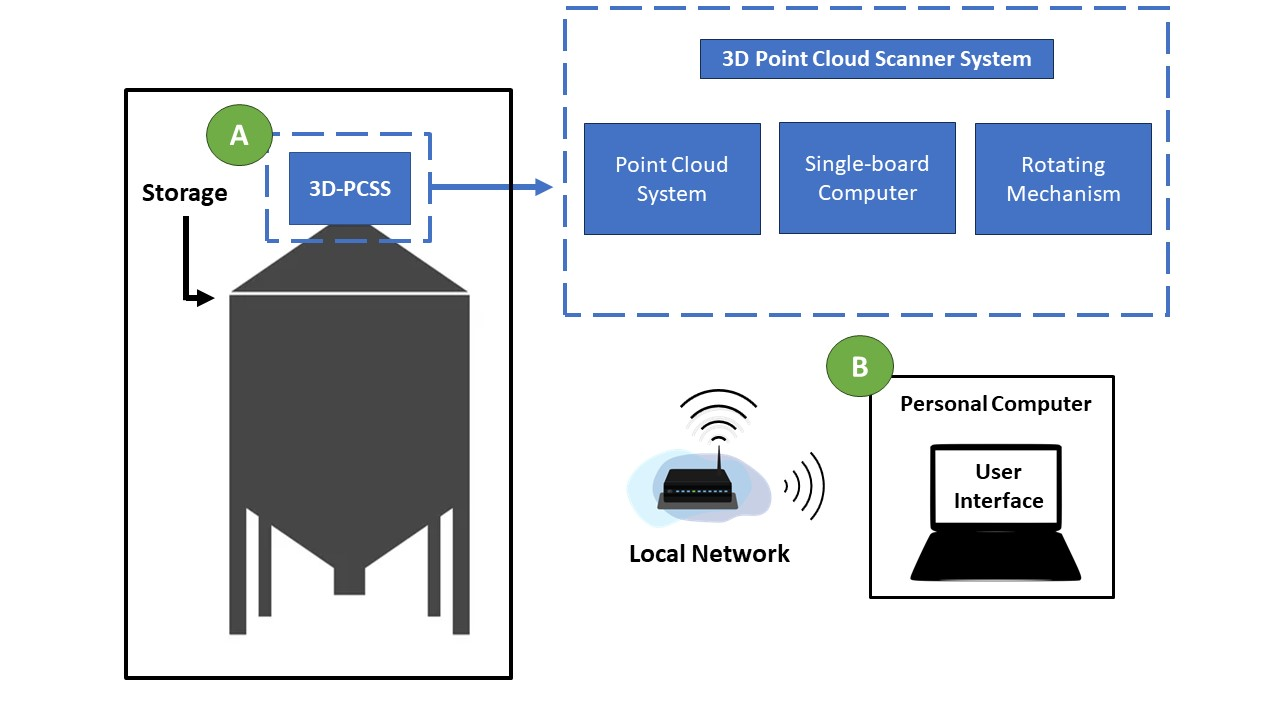
\includegraphics[width=1\textwidth]{Figures/system_analysis}
	\caption{Overall System Setup: (A) 3D-PCSS, (B) User Interface}
	\label{ch3:fig:overall_system_setup_development}
\end{figure}

\section{Hardware Development}
\label{ch3:sec:hardaware_design}

The hardware development conducted in this study involves the design and construction of 3D point cloud scanner. The system is divided in to two parts which discussed in the following subsection.

% The researcher will adopt the concept of tilting method using a 2D of-the-shelf LiDAR to acquire 3D point cloud data to minimize the cost compared to commercial 3D LiDAR. The hardware and physical components of 3D point cloud scanner are composed of three major components, the 2D LiDAR device, the tilting mechanism which include the fabricated holder for mechanical tilting and the motor for the rotation movement. In Figure \ref{ch3:fig:System Hardware Block Diagram}, the 3D point cloud scanner is placed at the top of the flour bin.

% \begin{figure}
% 	\centering
% 	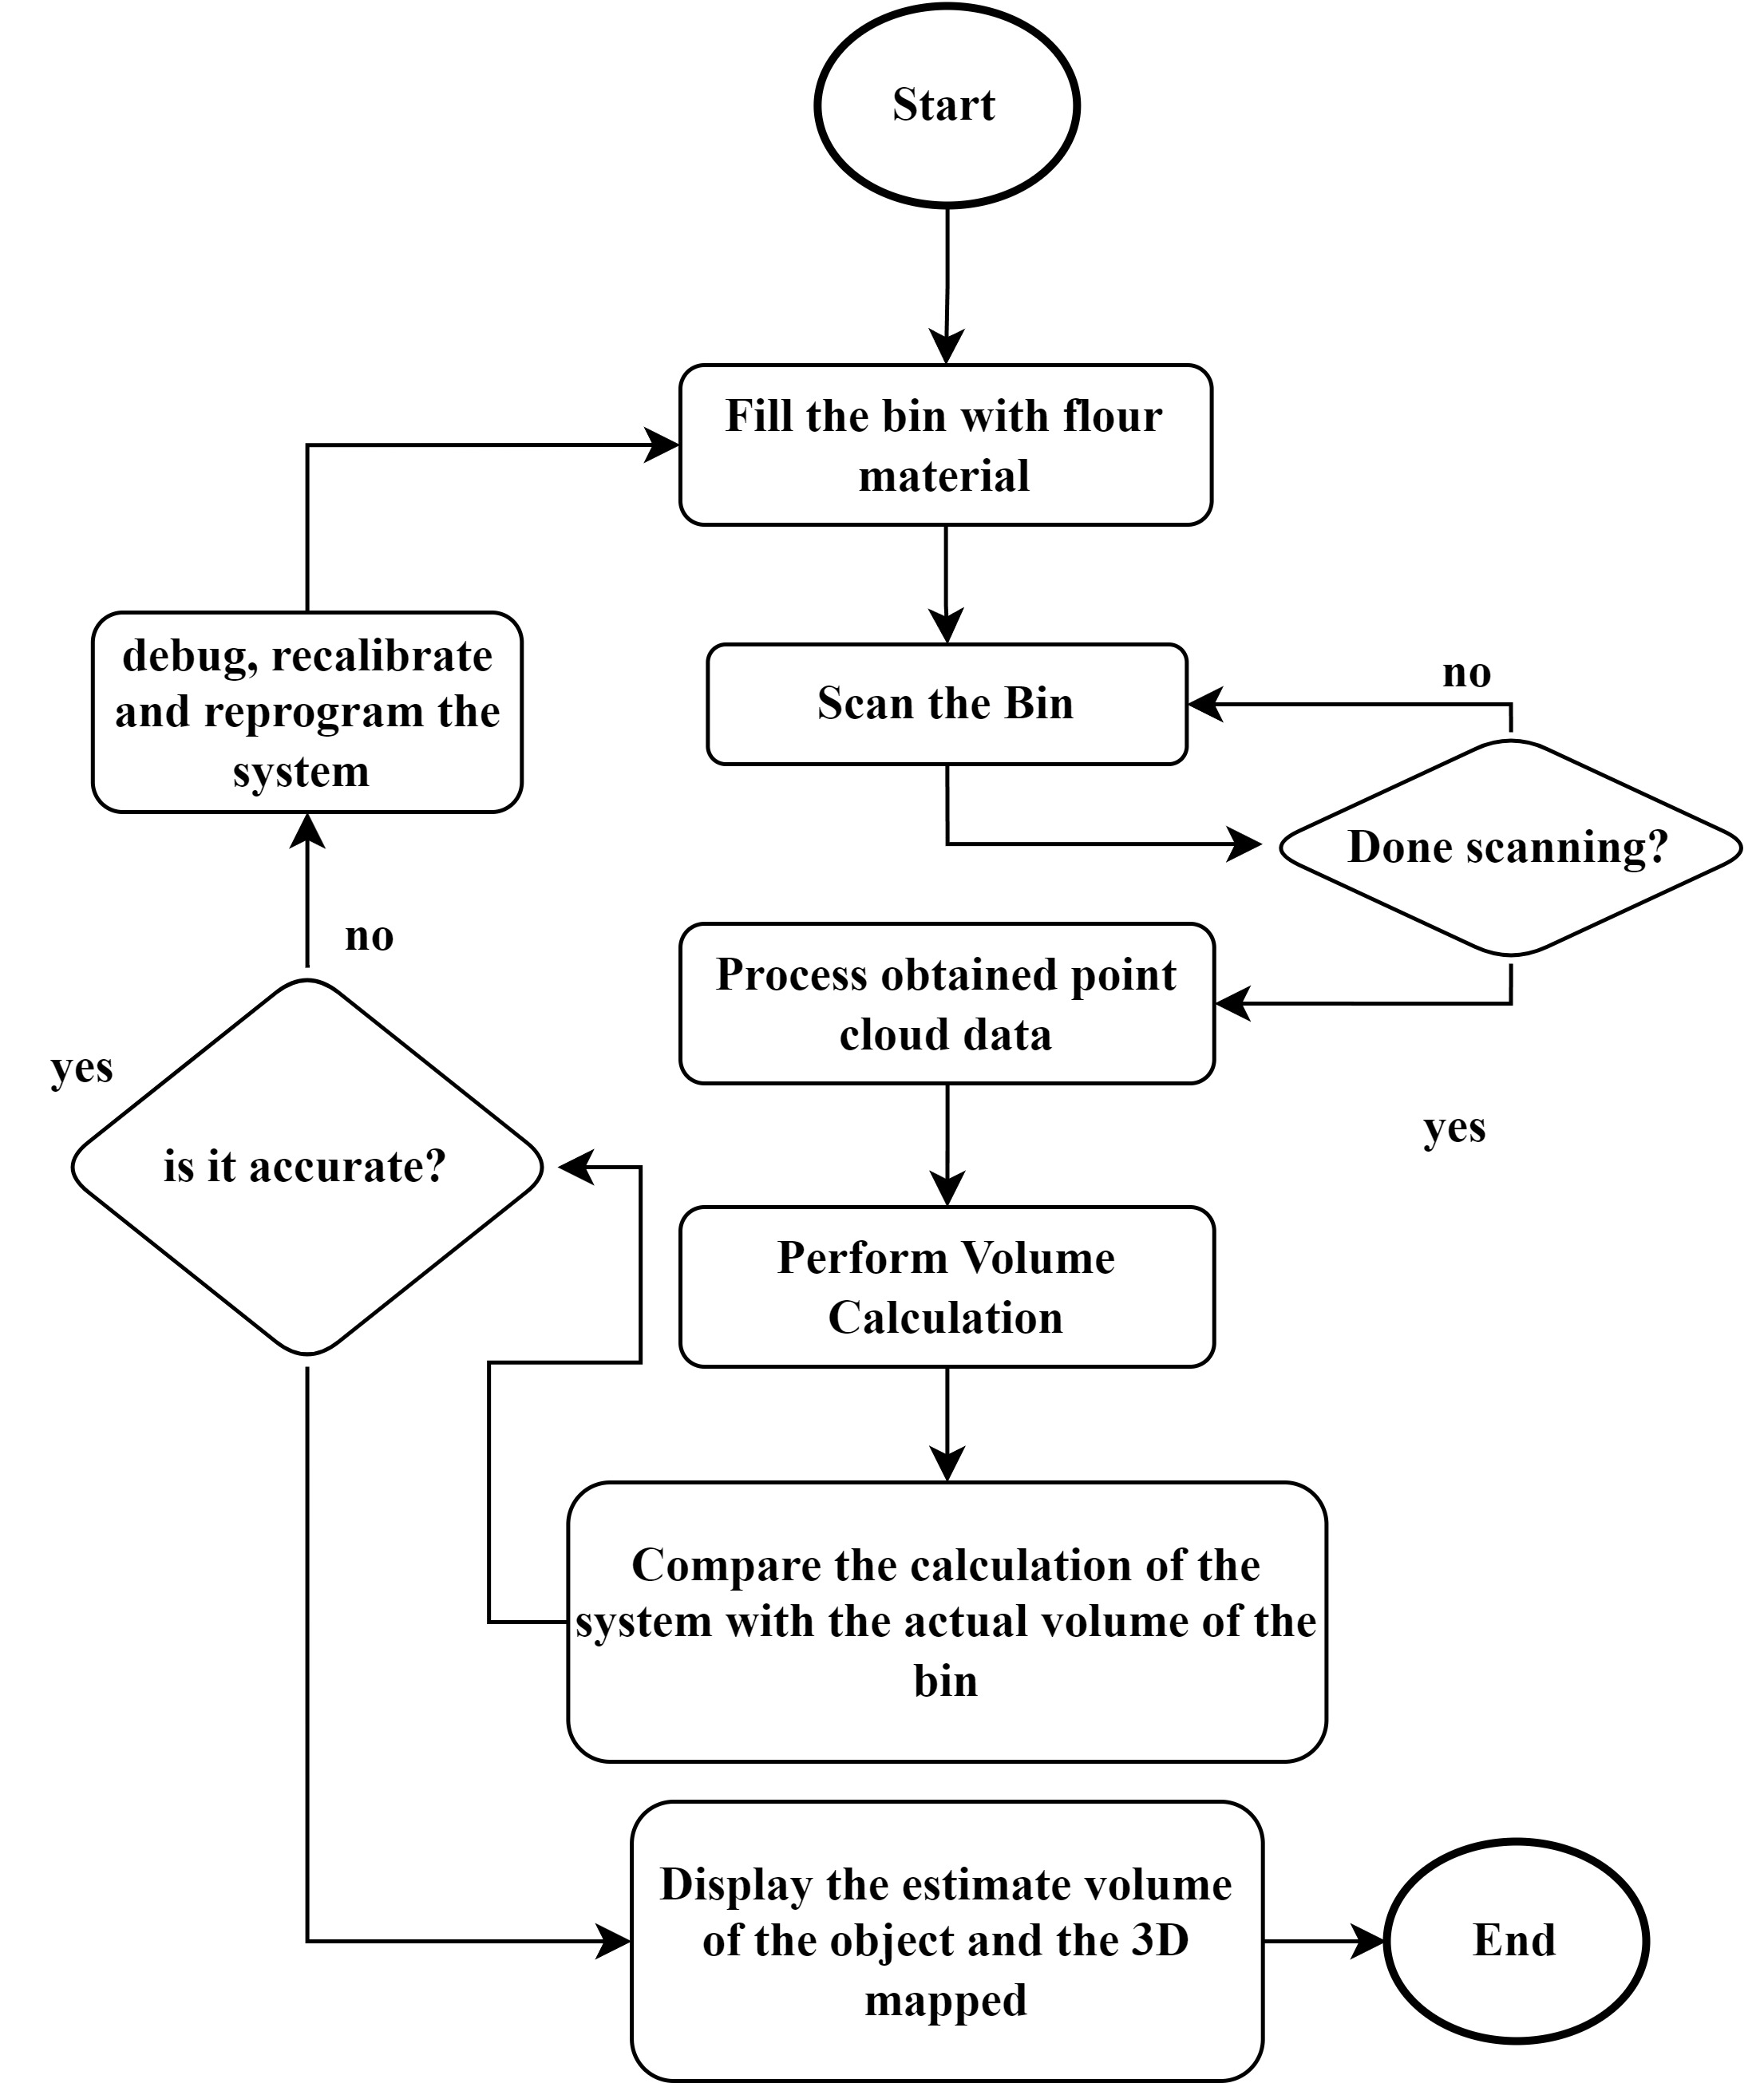
\includegraphics[width=0.9\textwidth]{Figures/general-flowchart-of-the-system-2.jpg}
% 	\caption{General Flowchart of the System}
% 	\label{ch3:fig:General flowchart of the system}
% \end{figure}

\subsection{3D Point Cloud Scanner Design (3D-PCSS)}
\label{ch3:subsec:3d_point_cloud_scanner_design}

The 3D-PCSS in this study considers the following design and functionality:
\begin{itemize}
	\item Based on low-cost 2D LiDAR device.
	\item Compact and portable for simplified installation.
	\item Support for connecting to a local network for remote data visualization and monitoring.
	\item Utilizing Robot Operating System (ROS) and Point Cloud Library (PCL) for adaptability development.
\end{itemize}

To achieve the design and functionality of the system mentioned, the development process, components and integration is discussed in the following section

\subsubsection*{Point Cloud Scanner System}

Point cloud devices, such as LiDAR (Light Detection and Ranging), offer exceptional accuracy in acquiring distance measurements over considerable distances. LiDAR systems emit laser pulses and measure the time it takes for these pulses to return after bouncing off objects in the environment. This technology enables the creation of highly detailed and accurate three-dimensional point clouds, which represent the surfaces and structures within the scanned area. Even low-cost LiDAR options are available in the market, making this technology accessible for various applications and budgets.

The point cloud scanner system in this study used a low-cost 2D LiDAR device controlled with single-board computer (SBC) for its computing functionality.

\subsubsection*{Rotating Mechanism}

The rotating mechanism design which is attached to the 2D LiDAR in this study is based on the methodology outlined in a previous research conducted by \citet{clar2022}. This prior study served as a foundational framework for the development of the rotating 2D LiDAR system in this study, providing into the integration of a pan-tilt unit (PTU) with a 2D LiDAR scanner to enable three-dimensional point cloud scanning. By employment the principles and techniques conducted in \citet{clar2022}, the current study aims to further refine and enhance the performance of the rotating 2D LiDAR system for its intended application and also address the problem encountered in the previous study.

% The servo motor utilized in this study is compatible with a Software Development Kit (SDK), which includes configurations for integration with the Robot Operating System (ROS). This feature enables communication and control of the servo motor within the ROS ecosystem, allowing for flexible and efficient development of robotic systems. This feature enables the LiDAR and Servo to communicate and synchronize, figure \ref{} illustrates the servo attached to the 2D LiDAR device to add additional axis. The figure shows the respective scan angle direction of the LiDAR and servo motor. The curial part of in this process is the synchronization process which in this study developed as shows in figure \ref{ch3:fig:servo_lidar_comm}. \\

The servo motor used in this study is compatible with a Software Development Kit (SDK) that includes configurations for integration with the Robot Operating System (ROS). This compatibility allows for communication and control of the servo motor within the ROS environment, facilitating the development of flexible and efficient robotic systems.

By employing this feature, the LiDAR and servo can communicate and synchronize. Figure \ref{ch3:fig:scan_and_movement_direction} illustrates how the servo is attached to the 2D LiDAR device to add an additional axis of movement. The figure also depicts the respective scan angle directions of the LiDAR and the movement direction servo motor.

Synchronization is a crucial aspect of this process. The synchronization method developed in this study is detailed in Figure \ref{ch3:fig:servo_lidar_comm}.

% \begin{algorithm}[]
% 	\caption{LDA}
% 	\label{ch3:algo:servo_and_lidar}
% 	\begin{algorithmic}[1]
% 		\FOR{$d$}
% 		\STATE{
% 			\FOR{$k\in\{1,...,K\}$}
% 			\STATE{Generate$\beta_k=(\beta_{k_1},...,\beta_{k,V})^T \sim Dirichlet(\cdot\vert\eta)$}
% 			\ENDFOR
% 		}
% 		\ENDFOR
% 	\end{algorithmic}
% \end{algorithm}

\begin{figure}[H]
	\centering
	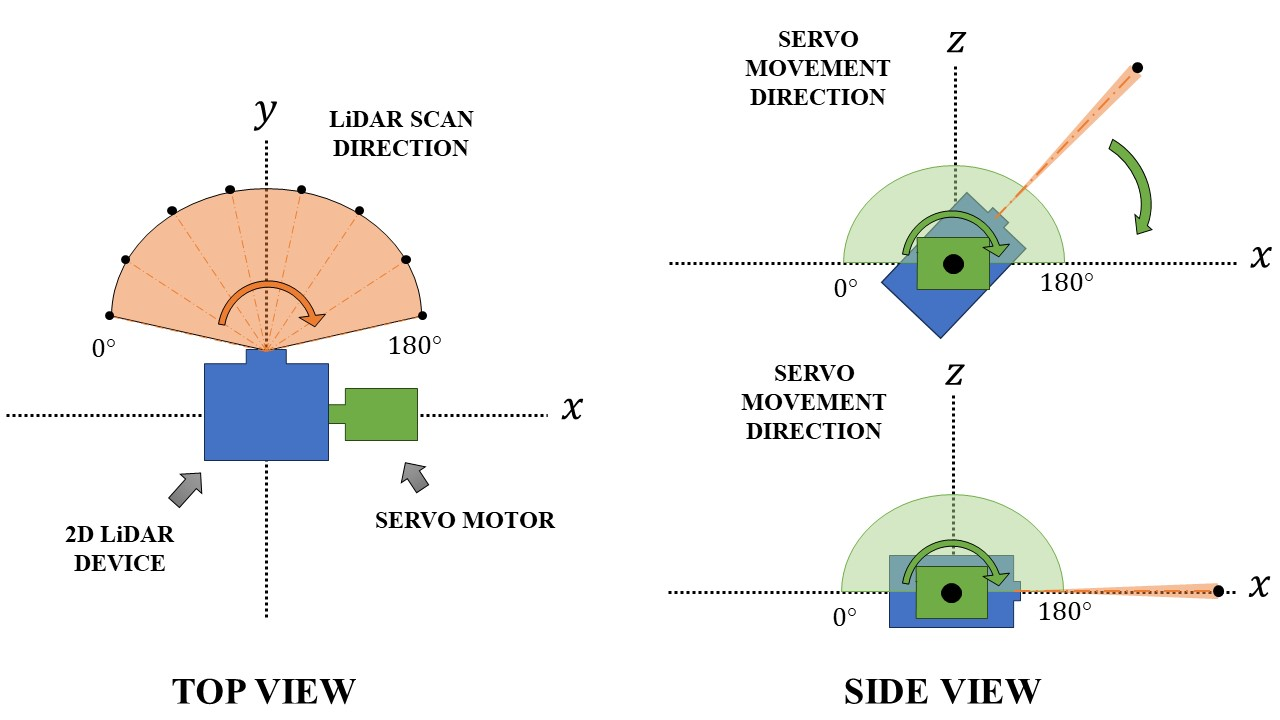
\includegraphics[width=1\textwidth]{Figures/scan_direction_of_lidar_and_servo}
	\caption{Scan Direction of LiDAR and Movement Direction of the Servo}
	\label{ch3:fig:servo_lidar_comm}
\end{figure}

\begin{figure}[H]
	\centering
	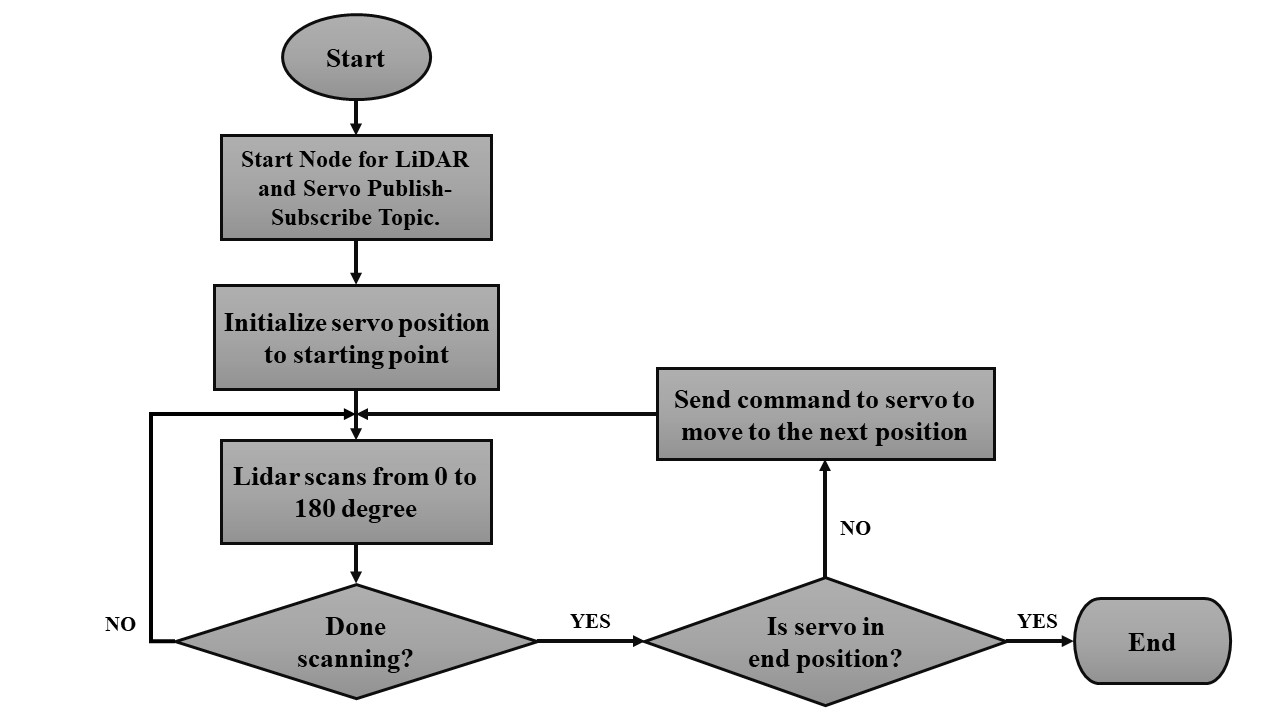
\includegraphics[width=1\textwidth]{Figures/servo_lidar_comm}
	\caption{Synchronization Process of LiDAR and Servo}
	\label{ch3:fig:scan_and_movement_direction}
\end{figure}

In figure \ref{ch3:fig:components_of_3d-pcss}, the components of the point cloud scanner and rotating device are integrated to develop a 3D point cloud scanner system. These individual components are divided into four categories, as shown in figure \ref{ch3:fig:block-digram-connection}: sensor, control, actuator, and power. The double-headed arrow indicates a two-way communication from and to the control device. Lastly, the hardware design flow chart of the system is shown in figure \ref{ch3:fig:3d-pcss_development_flow_chart}.

\begin{figure}[H]
	\centering
	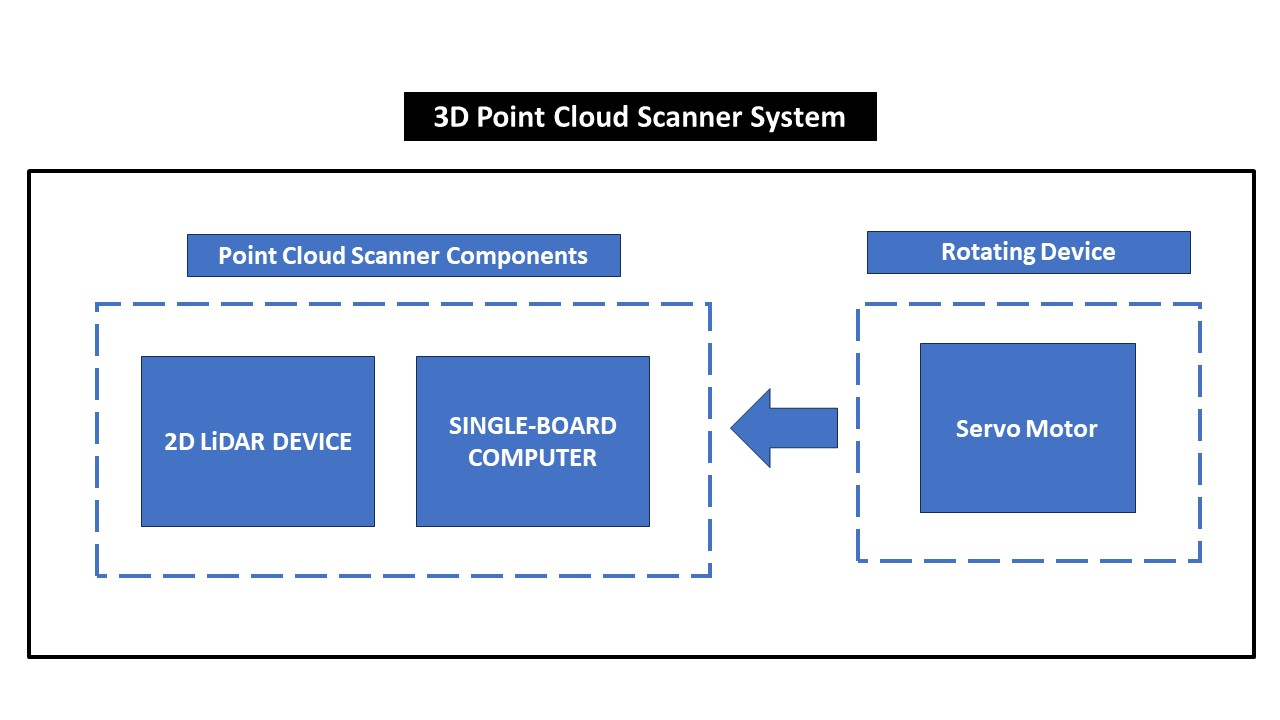
\includegraphics[width=1\textwidth]{Figures/3D-PCSS components}
	\caption{Major Components of 3D-PCSS}
	\label{ch3:fig:components_of_3d-pcss}
\end{figure}

\begin{figure}[H]
	\centering
	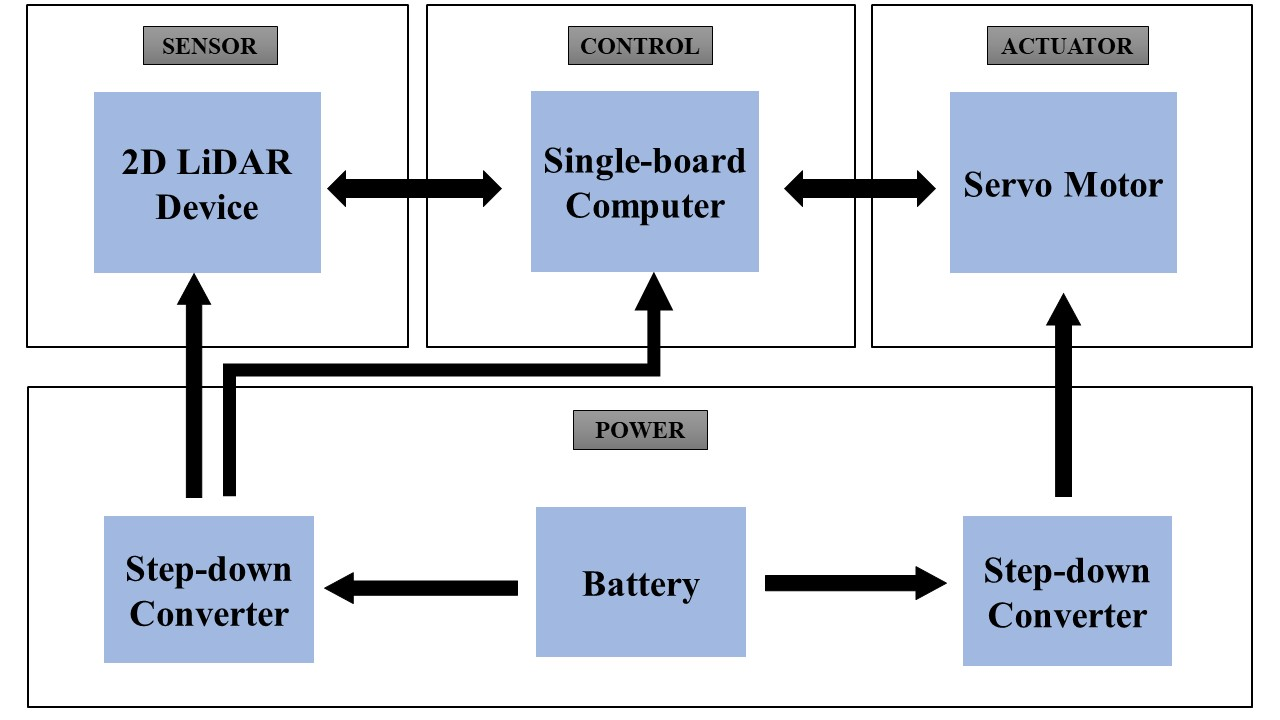
\includegraphics[width=1\textwidth]{Figures/components-block-diagram}
	\caption{Block Diagram Connection of the Components}
	\label{ch3:fig:block-digram-connection}
\end{figure}


\begin{figure}[H]
	\centering
	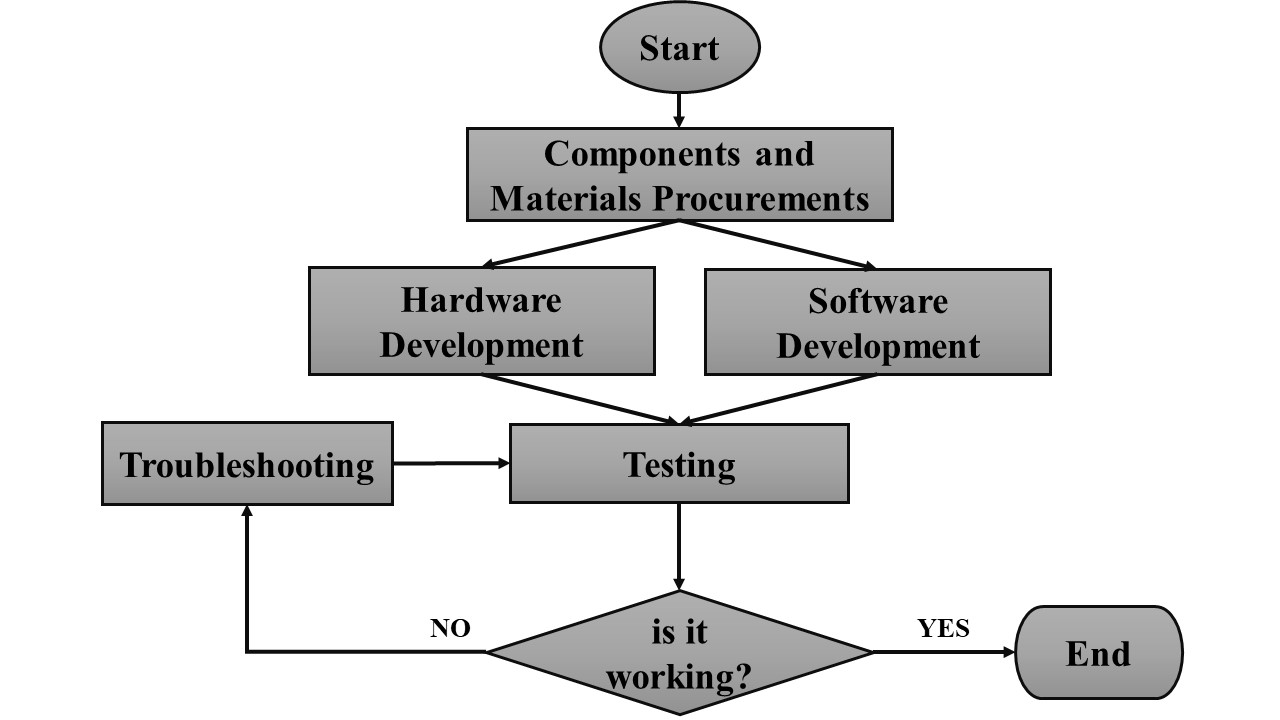
\includegraphics[width=0.8\textwidth]{Figures/hardware_flowchart}
	\caption{Hardware Design Flow Chart}
	\label{ch3:fig:3d-pcss_development_flow_chart}
\end{figure}

% \subsection{Data Gathering}
% For the data gathering of the raw point cloud, all the major hardware of the system will be assemble and integrate as shown in Figure \ref{ch3:fig:System Hardware Block Diagram}. The scanned data from the 2D LiDAR sensor will be received by small computer which is Raspberry Pi for the processing of the raw data. This small computer is connected to the internet in order to control remotely by the personal laptop. Different scanning procedure will be performed to gather point cloud data.

% \begin{figure}[H]
% 	\centering
% 	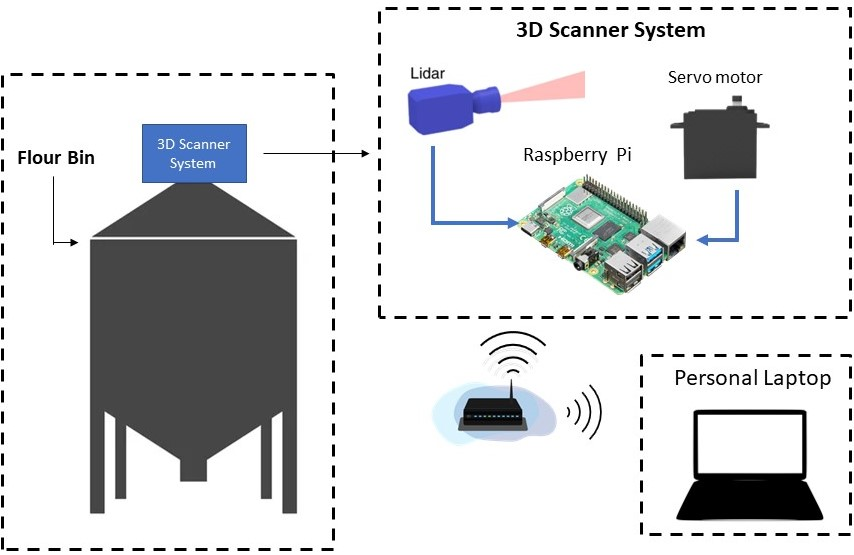
\includegraphics[width=0.9\textwidth]{Figures/system-hardware-block-diagram.jpg}
% 	\caption{System Hardware Block Diagram}
% 	\label{ch3:fig:System Hardware Block Diagram}
% \end{figure}

\section{Software Development}
\label{ch3:sec:firmware_development_design}

Software design plays a crucial role in the development of the 3D-PCSS by facilitating communication between hardware components, and allows connection with external software system. The system was designed to initialize all necessary components, including nodes and connection, immediately upon power-up. This ensures seamless operation and also establish connection with the developed web application for user interaction. As described in figure \ref{ch3:fig:software_system_process}, after turning on the system, it initializes essential nodes and enter in idle mode waiting for an external command coming from the web application. The system remain in idle mode unless turnoff. The development of software processes, including the choice of operating system and frameworks is outlined in this section.

Throughout this study, it's important to note that the terms 'process' and 'nodes' are used interchangeably. This interchangeable usage highlights the fundamental concept in ROS where processes, represented as nodes, perform computation and communication tasks within the system.

\begin{figure}[H]
	\centering
	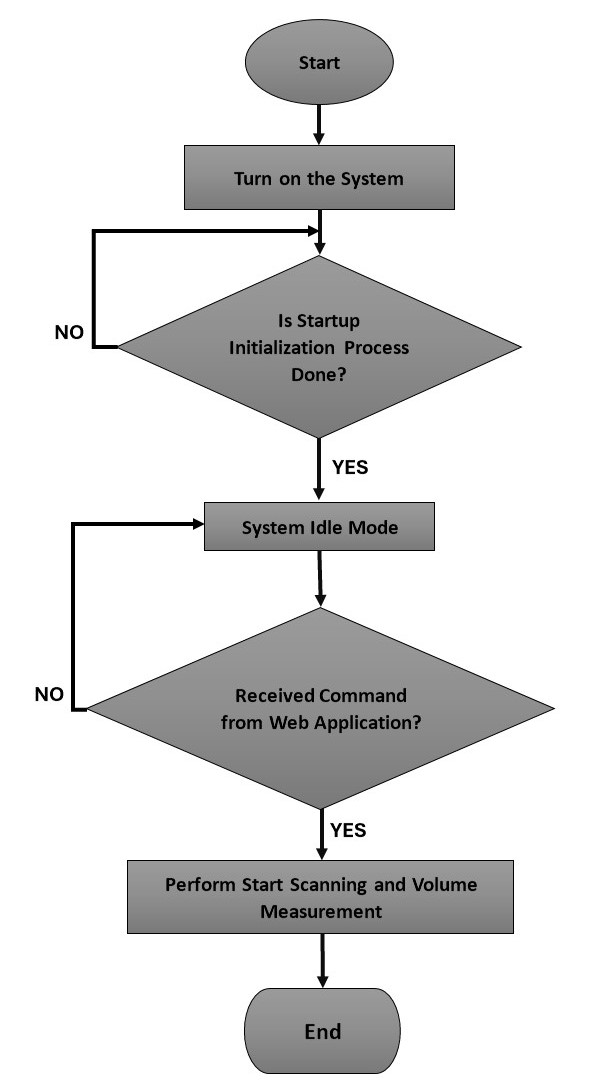
\includegraphics[width=0.7\textwidth, height=0.7\textheight]{Figures/software_system_process}
	\caption{System Idle Mode Process Flow Chart}
	\label{ch3:fig:software_system_process}
\end{figure}

\subsection{Operating System and Frameworks}

In this study, the single-board computer (SBC) used in the 3D-PCSS requires an appropriate OS and frameworks to support the execution of firmware and software components. Linux-based operating systems, such as Ubuntu, is commonly chosen for SBCs due to its reliability, flexibility, and extensive community support. This OS option provide a stable platform for running Robot Operating System (ROS) nodes and managing system resources effectively, thus, was utilized in this study. ROS framework was also utilized in this study to develop a publish-subscribe relationship between ROS nodes. Lastly, Point Cloud Library (PCL) serves in this study as a fundamental library being used for processing and analyzing point cloud data. PCL provides a comprehensive set of algorithms and tools for tasks such as point cloud registration, filtering and computational geometry to name a few.

\subsection{Startup Initialization Process}
Roscore and rosgridge are the two essential cores that used in the software of 3D-PCSS. These cores or nodes typically need to be executed manually through the command-line interface (CLI) or desktop environment terminal to run and process data, or to initiate other nodes and do specific tasks. However, it is impractical to start and stop this nodes each time the system is turn on or off, thus, in this study a custom service file was developed to automate and start these nodes after the system is turn on. This file is created using Linux systemd to configure and instantly run the cores.

% The Raspberry Pi will receive the scanned raw data coming from the 3D point cloud scanner. This data will be processed in different stages to produced desired output, such as point cloud pre-processing (formatting, converting, clustering, and cleansing) and post-processing (e.g., 3D mapping and volume measurement). Various platforms and frameworks nowadays are available to ease the handling of these massive raw data, thus, formatting the data to a desired platform must be perform. Typically, the value of raw data coming from the LiDAR sensor is not directly a point cloud data but rather a value of the distance between the sensor and the reflected nearest object in a particular direction, therefore, the data is converted into point cloud which composed of x, y, and z values. The Equation \eqref{ch3:eq:x-point}, \eqref{ch3:eq:y-point}, and \eqref{ch3:eq:z-point} is conversion of polar coordinates (distance, angle) to cartesian coordinates x, y, and z, respectively, in a 3D coordinate system.

% \begin{equation}
% 	x_{point_{i}} = \ \sin(i) \times d \
% 	\label{ch3:eq:x-point}
% \end{equation}
% \begin{equation}
% 	y_{point_{i}} = \ \cos(\pi) \times \cos(i) \times d \
% 	\label{ch3:eq:y-point}
% \end{equation}
% \begin{equation}
% 	z_{point_{i}} = \ -\cos(i) \times \sin(\pi) \times d \
% 	\label{ch3:eq:z-point}
% \end{equation}

% Where:

% \indent \indent i = scan angle of the scanner

% \indent \indent d = the distance point of the emitted pulse by the LiDAR (meter)

\subsection{System Scanning and LiDAR Range Values Processes}
As described in figure \ref{ch3:fig:overall_system_setup_development}, the system is placed at the top of the storage bin. Once the system receive a command from the web application, it will start scanning the inside of the storage bin and acquiring ranges values from the LiDAR as discussed in figure \ref{ch3:fig:software_system_process}. The study developed a ros nodes that handle different processes such as initialization of the LiDAR device and servo motor, establishing a publish-subscribe relationship between these devices, and the conversion of LiDAR range scan data to point cloud data. The raw scan data from the LiDAR are typically range values of the return pulses. These range values enters different stages of pre-processes to be mapped in two- or three-dimensional Euclidean space to create a point cloud data and use for further post-processing. The flow of the processes from initialization to mapped point cloud data is illustrated in this figure \ref{ch3:fig:scanning-to-pc-flow-chart} The method used in this study for processing the ranges values gathered from the LiDAR device is described in the figure \ref{ch3:fig:point_cloud_conversion}.  $\rho$ translates to the distance from the origin $(0,0,0)$, which is the in our case the LiDAR, and this distance is measured as meter. The angle $\theta$ is the rotation around the z-axis in the xy-plane. The angle $\phi$ is the tilt of the radius vector from the positive z-axis, it goes from 0 degree at the positive z-axis down to 90 degree at the xy-plane and all the way down to 180 degree on the negative z-axis. Equation \ref{ch3:eq:x}, \ref{ch3:eq:y} and \ref{ch3:eq:z} shows the X, Y, and Z conversion formula respectively.

\begin{figure}[H]
	\centering
	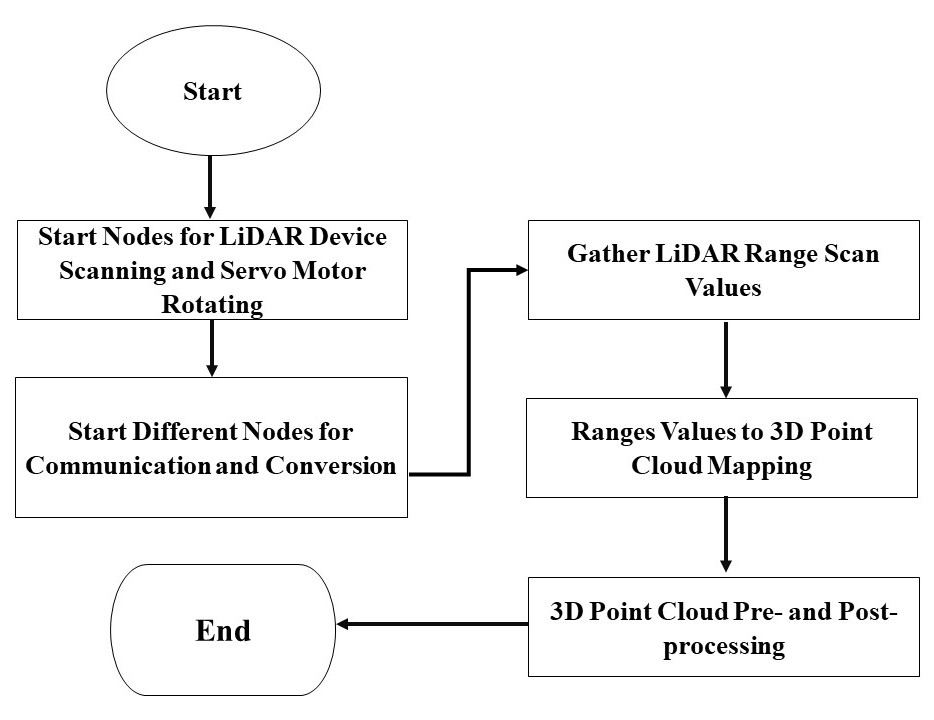
\includegraphics[width=0.9\textwidth]{Figures/scanning-to-pc-flow-chart}
	\caption{From Scanning to Mapped Point Cloud Data Flow Chart}
	\label{ch3:fig:scanning-to-pc-flow-chart}
\end{figure}

\begin{equation}
	\label{ch3:eq:x}
	x = \rho \times \sin(\theta) \times \cos(\phi)
\end{equation}
\begin{equation}
	\label{ch3:eq:y}
	y = \rho \times \sin(\theta) \times \sin(\phi)
\end{equation}
\begin{equation}
	\label{ch3:eq:z}
	z = \rho \times \cos(\theta)
\end{equation}

\begin{figure}[H]
	\centering
	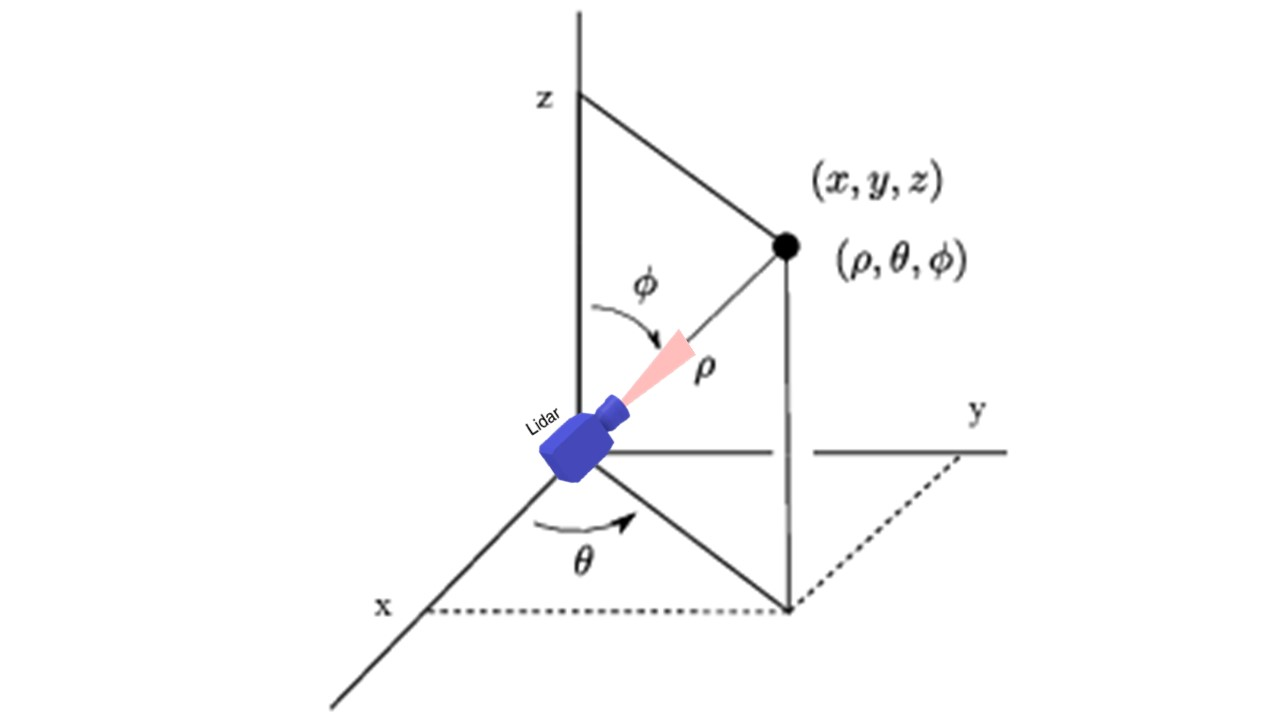
\includegraphics[width=1\textwidth]{Figures/point cloud conversion}
	\caption{LiDAR Scan Range Conversion from Polar Coordintes $(\rho,\theta,\phi)$, to Cartesian Coordinate $(x,y,z)$}
	\label{ch3:fig:point_cloud_conversion}
\end{figure}

\subsection{Point Cloud Data to Measured Volume}
\label{ch3:sec:Volume Estimation}
An Empty-space approached was used to measured the flour materials inside the storage bin. A simple representation of an empty-space approach is illustrated in figure \ref{ch3:fig:volume-estimation-figure}. The 3D-PCSS is place at the top of the storage bin to scan the empty space and generate point cloud data. These point cloud data is process to calculate the the empty space volume using Convex Hull method. Theoretically, the volume of the flour materials is determined by subtracting the empty space volume from the bin's maximum volume capacity as it is also a commonly used method in these studies \citet{raba2020,clar2022}.

\begin{figure}[H]
	\centering
	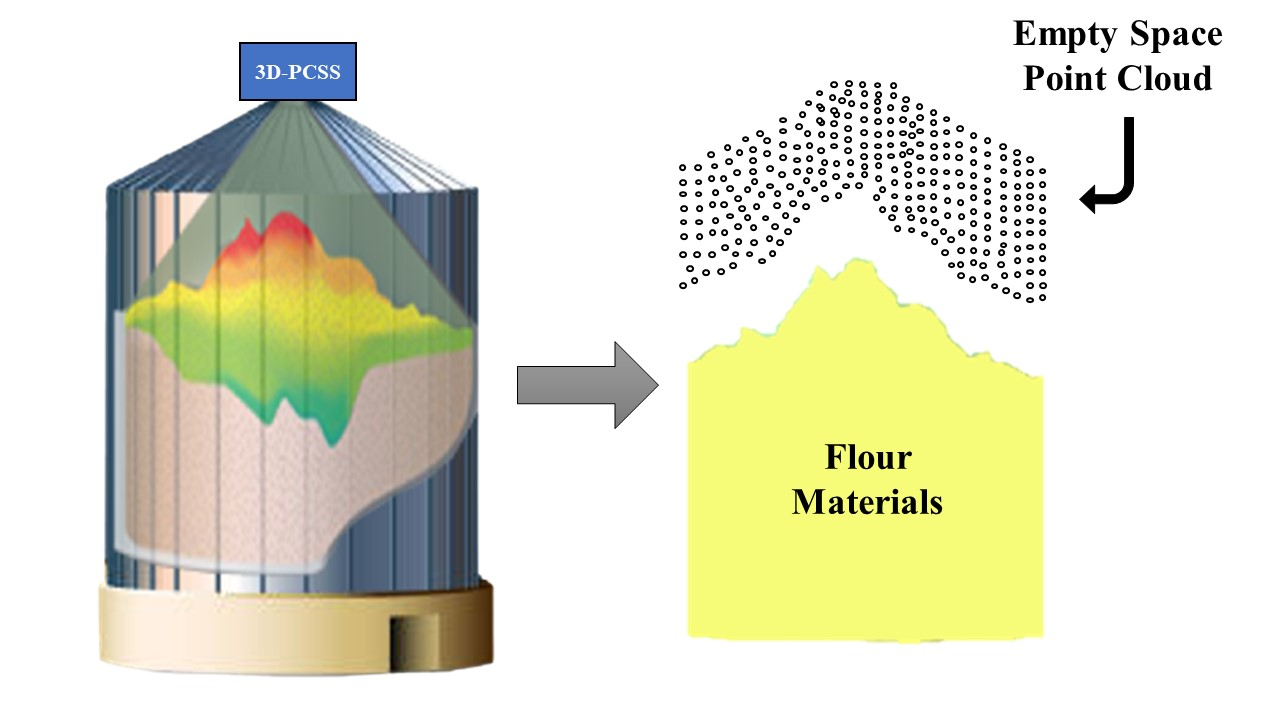
\includegraphics[width=1\textwidth]{Figures/empty_space}
	\caption{System Scanning (right), Generated Empty Space Point Cloud Data (left)}
	\label{ch3:fig:volume-estimation-figure}
\end{figure}

% \section{Web-based Application Development}
% This custom user interface based on web application is developed to used for the 3D-PCSS. The tools, framework and and resources of the system is discussed in this section.

% \subsection{}

% The user interface consider the following design and functionality, the UI should be:
% \begin{itemize}
% 	\item Intuitive and simple.
% 	\item Able to establish connection to the 3D-PCSS.
% 	\item Able to send command, display 3D point cloud data and volume measurement.
% \end{itemize}


\section{Web-based Application Development}
This section covers the process of developing the custom user interface for the 3D-PCSS utilizing web application. The flow of the connection of the web application connecting to the 3D-PCSS is presented in the figure \ref{ch3:fig:web_app_connection}. The system and the web application is within the same local network, thus after entering the local and port address in the web application, the web socket connection can be established and can send command to the system.

The user interface consider the following design and functionality, the UI should be:
\begin{itemize}
	\item Intuitive and simple.
	\item Able to establish connection to the 3D-PCSS.
	\item Able to send command, display 3D point cloud data and volume measurement.
\end{itemize}

\begin{figure}[H]
	\centering
	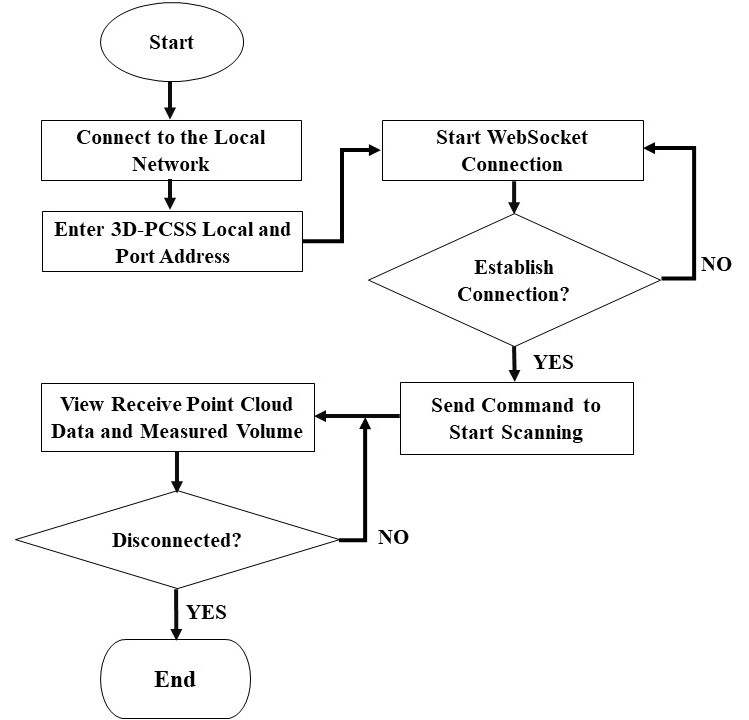
\includegraphics[width=0.9\textwidth]{Figures/web_app_connection}
	\caption{Web Application Connection Process Flow Chart}
	\label{ch3:fig:web_app_connection}
\end{figure}

\subsection{Communication Protocol}
The web-based interface and 3D-PCSS utilizes WebSocket communication protocol. This communication uses full-duplex channels to establish over a single TCP connection. It allows for less latency than typical HTTP connections when a client and server interact. Within the framework of ROS applications, WebSocket enables bi-directional, real-time communication, enabling servers to rapidly transmit updates to clients. The figure \ref{ch3:fig:websocket-connection} demonstrate the initialization of the Websocket communication between the web interface and the 3D-PCSS. The following step to establish this communication is explain below:

\begin{enumerate}
	\item \textbf{The Client Makes a Request:} The WebSocket client initiates the handshake by sending an HTTP request to the server.
	\item \textbf{The Server Accepts the Request:} If the server is willing to establish a WebSocket connection, it responds with an HTTP response that has a status code of 101 (Switching Protocols).
	\item \textbf{WebSocket Connection Established:} Once both the client and server have exchanged their handshake messages, the WebSocket connection is established. Data can now flow bidirectionally between the client and server over the single TCP connection.
\end{enumerate}

\begin{figure}[H]
	\centering
	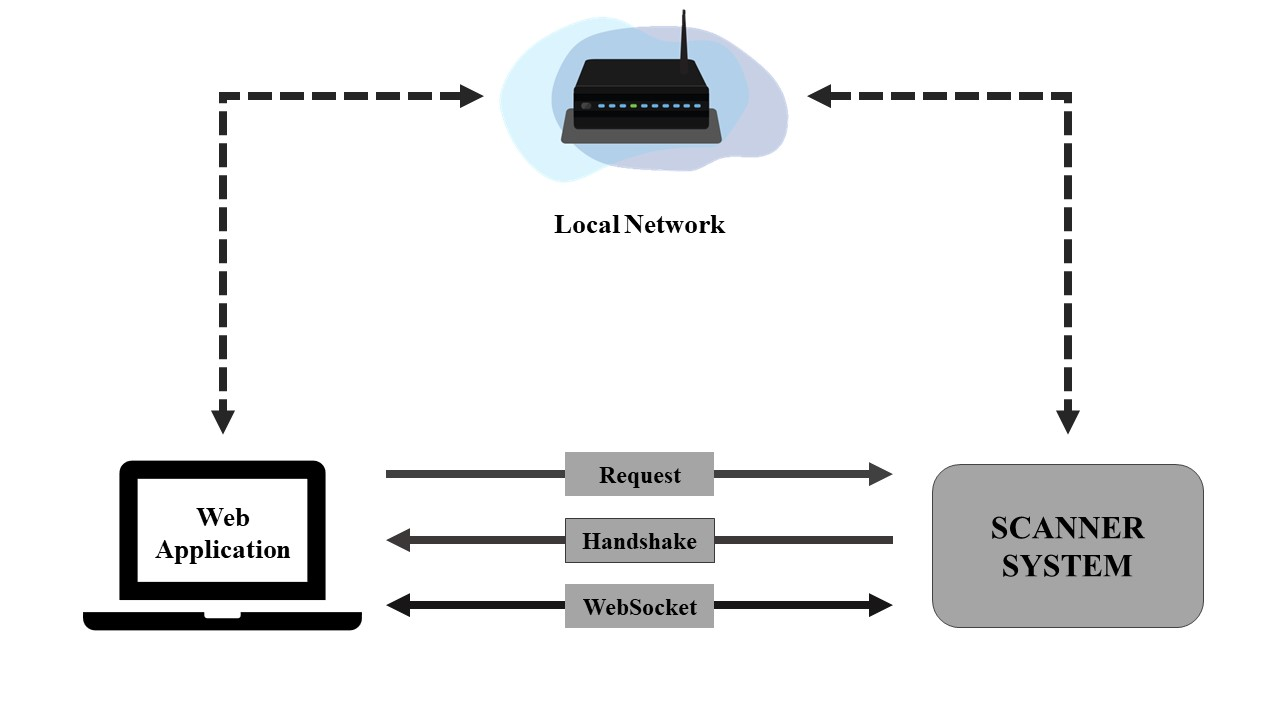
\includegraphics[width=0.9\textwidth]{Figures/websocket-connection}
	\caption{Communication Protocol of the Web Interface and the System}
	\label{ch3:fig:websocket-connection}
\end{figure}

\section{Overall System Testing and Evaluation}
\label{ch3:sec:TestingAndEvaluation}

In this section, various tests were conducted to evaluate the performance of the overall system. After successful development and integration of the system and web application, they were tested and evaluated for accuracy and functionality.

\subsection{Constructing of Storage Bin}
\label{ch3:subsec:Modeling of Flour Bin}
To test the performance and accuracy of the overall system, the study involves constructing a mock-up flour storage bin modeled after those commonly used in food manufacturing industries. The mock-up bin is designed to closely mimic the geometric shape and proportions of real storage bins used in practice. The CAD model design, shown in figure \ref{ch3:fig:cad_storage_bin}, serves as the guide for the physical construction. The design is composed of rectangular shape and conical frustum underneath. The CAD design of rectangular shape has a dimension of 2.5 meters in height, 0.5 meters in length, and 0.69 meters in width. The conical frustum, which is tapers from the base of the rectangular section, has a top radius of 0.21 meters, a bottom radius of 0.17 meters and height of 0.21 meters. The 3D-PCSS was placed at the top of created mock-up storage bin for test and evaluation.

\begin{figure}[H]
	\centering
	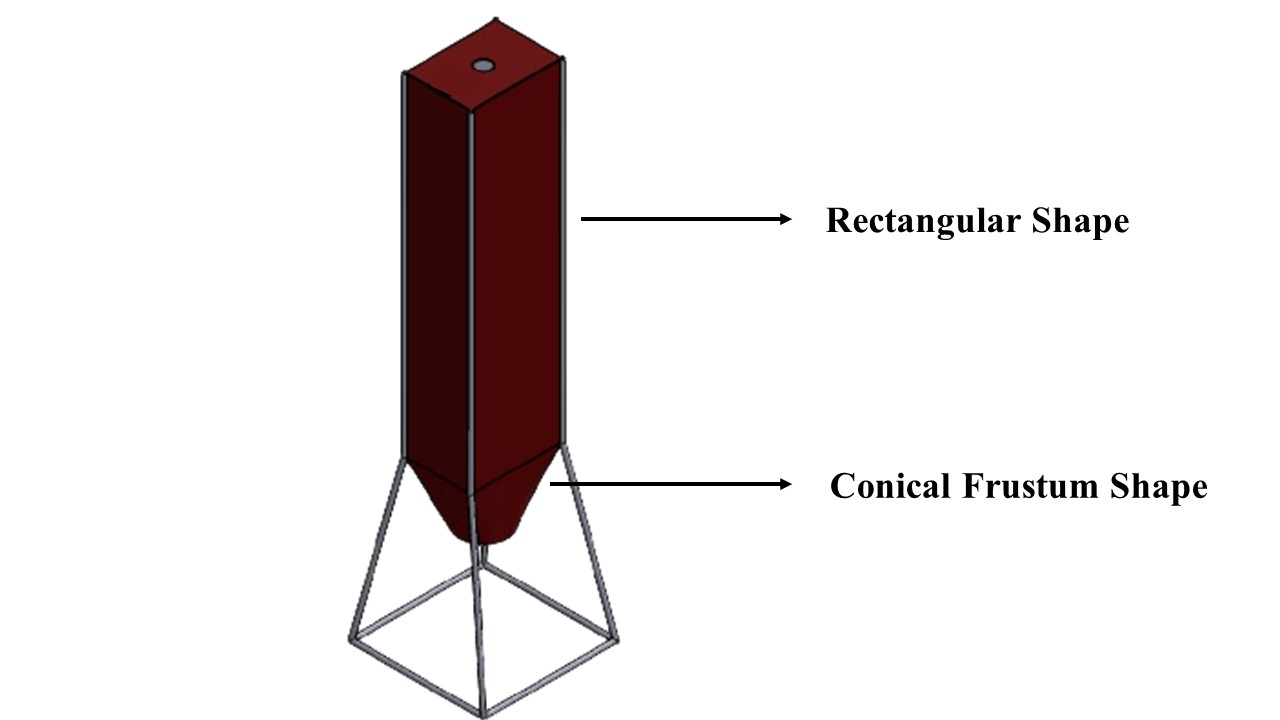
\includegraphics[width=1\textwidth]{Figures/cad_storage_bin}
	\caption{CAD Model Design of the Storage Bin}
	\label{ch3:fig:cad_storage_bin}
\end{figure}

\subsection{Different Testing Case Procedure}
\label{ch3:subsec:Different Testing Procedure}
The study conducted different tests and evaluations to observe the accuracy and performance of the overall system. The study performed multiple tests to assess and validate the accuracy and effectiveness of the developed method, and each of tests had multiple trials. The different testing procedures of the system were as follows:

\subsection*{Test Case 1: Empty Storage Bin Scanning}

In this test case, multiple scans of an empty storage bin were conducted. This involved performing 30 or more scanning trials. By comparing the system's measured volume with the actual volume capacity of the storage bin, the test aimed to validate the overall system's performance and accuracy. This test also provided a baseline for assessing the performance of the developed method.

\subsection*{Test Case 2: Filling the Storage Bin with Known Volume}

The second test case involved filling the storage bin with flour using containers of known volume. Three specific scenarios were conducted, each with different percentages of the storage bin's maximum capacity, along with known volumes and two different flour surface contour:

\begin{enumerate}
	\item The storage bin was filled up to 5.8\% of its maximum capacity, with a known volume of 0.0594 cubic meters.
	\item The storage bin was filled up to 47.2\% of its maximum capacity, with a known volume of 0.4752 cubic meters.
	\item The storage bin was filled up to 70.37\% of its maximum capacity, with a known volume of 0.7128 cubic meters.
\end{enumerate}

These different test cases were designed to assess the accuracy and performance of the overall system.

% These test cases were crucial in evaluating the accuracy and performance of the system under different conditions.
% \subsection{Evaluation of the System}
% \label{ch3:subsec:Evaluation of the System}
% Based on the conducted different testing mentioned in \ref{ch3:subsec:Different Testing Procedure}, the researcher will evaluate the conducted testing based on the volume of scanned data. System in the following evaluation

% To evaluate the testing \ref{ch3:first}, the researcher will measure the accuracy of the system by comparing the estimated volume of the system  with the actual volume of the different shape of the bin, calculate the error percentage for each trial and assess the over all precision of the system. Table \ref{ch3:tab:Testing 1} shows the sample comparison of the testing.

% \begin{table}[H]
% 	\caption{Testing \ref{ch3:first}}
% 	\label{ch3:tab:Testing 1}
% 	\centering
% 	\begin{tabular}{|c|c|c|c|}
% 		\hline
% 		% First row
% 		Flour bin Shape & Actual Volume (\si{mm^3}) & Scanned Volume (\si{mm^3}) & Error (\%) \\
% 		\hline
% 		\multicolumn{4}{|c|}{Trial 1}                                                         \\
% 		\hline
% 		% Second row
% 		Cube            & -                         & -                          & -          \\
% 		\hline
% 		% Third row
% 		Cylinder        & -                         & -                          & -          \\
% 		\hline
% 		\multicolumn{4}{|c|}{Trial 2}                                                         \\
% 		\hline
% 		Cube            & -                         & -                          & -          \\
% 		\hline
% 		% Third row
% 		Cylinder        & -                         & -                          & -          \\
% 		\hline
% 	\end{tabular}
% \end{table}

% Testing \ref{ch3:second} will be evaluated from the testing \ref{ch3:first} based on the number of point cloud acquired of both testing, and compare it. Basically, the testing \ref{ch3:second} will acquired more point cloud compared to testing \ref{ch3:first} due to multi-echo or multiple returning from the dust and the flour bin.

% In testing \ref{ch3:third} and \ref{ch3:fourth}, the researcher will place flour materials inside the bin with different surface shape and perform volume estimation. After the volume estimation, the researcher will generate dust, scan the bin, perform volume estimation and compare it to the result of the testing \ref{ch3:third}. The sample result of testing \ref{ch3:third} and \ref{ch3:fourth} is shown in table

% \begin{table}[H]
% 	\caption{Testing 3 and 4}
% 	\label{ch3:tab:Testing 3 and 4}
% 	\centering
% 	\begin{tabular}{|c|p{0.27\linewidth}|p{0.26\linewidth}|p{0.2\linewidth}|}
% 		\hline
% 		% First row
% 		Flour bin Shape & Scanned Volume (without dust) & Scanned Volume (with dust) & Error (\%) \\
% 		\hline
% 		\multicolumn{4}{|c|}{Surface Shape 1}                                                     \\
% 		\hline
% 		% Second row
% 		Cube            & -                             & -                          & -          \\
% 		\hline
% 		% Third row
% 		Cylinder        & -                             & -                          & -          \\
% 		\hline
% 		\multicolumn{4}{|c|}{Surface Shape 2}                                                     \\
% 		\hline
% 		Cube            & -                             & -                          & -          \\
% 		\hline
% 		% Third row
% 		Cylinder        & -                             & -                          & -          \\
% 		\hline
% 	\end{tabular}
% \end{table}